\subsection{Microcontroller}
A microcontroller is a self-contained system with peripherals, memory and a processor that can be used as an embedded system. Most programmable microcontrollers that are used today are embedded in other consumer products or machinery including phones, peripherals, automobiles and household appliances for computer systems. Due to that, another name for a microcontroller is "embedded controller." Some embedded systems are more sophisticated, while others have minimal requirements for memory and programming length and a low software complexity. Input and output devices include solenoids, LCD displays, relays, switches and sensors for data like humidity, temperature or light level, amongst others.\\
Microcontrollers are used in automatically controlled products and devices, such as automobile engine control systems, implantable medical devices, remote controls, office machines, appliances, power tools, toys and other embedded systems. By reducing the size and cost compared to a design that uses a separate microprocessor, memory, and input/output devices, microcontrollers make it economical to digitally control even more devices and processes. Mixed signal microcontrollers are common, integrating analog components needed to control non-digital electronic systems.
\subsubsection{Embedded Design}
A microcontroller can be considered a self-contained system with a processor, memory and peripherals and can be used as an embedded system. The majority of microcontrollers in use today are embedded in other machinery, such as automobiles, telephones, appliances, and peripherals for computer systems.\\
While some embedded systems are very sophisticated, many have minimal requirements for memory and program length, with no operating system, and low software complexity. Typical input and output devices include switches, relays, solenoids, LEDs, small or custom liquid-crystal displays, radio frequency devices, and sensors for data such as temperature, humidity, light level etc. Embedded systems usually have no keyboard, screen, disks, printers, or other recognizable I/O devices of a personal computer, and may lack human interaction devices of any kind.
\subsubsection{Programming Environment}
Microcontrollers were originally programmed only in assembly language, but various high-level programming languages, such as Python and JavaScript, are now also in common use to target microcontrollers and embedded systems.These languages are either designed specially for the purpose, or versions of general purpose languages such as the C programming language. Compilers for general purpose languages will typically have some restrictions as well as enhancements to better support the unique characteristics of microcontrollers. Some microcontrollers have environments to aid developing certain types of applications.\\
Simulators are available for some microcontrollers. These allow a developer to analyze what the behavior of the microcontroller and their program should be if they were using the actual part. A simulator will show the internal processor state and also that of the outputs, as well as allowing input signals to be generated. While on the one hand most simulators will be limited from being unable to simulate much other hardware in a system, they can exercise conditions that may otherwise be hard to reproduce at will in the physical implementation, and can be the quickest way to debug and analyze problems.
\subsubsection{Types of microcontrollers}
As of 2008, there are several dozen microcontroller architectures and vendors including:
\begin{enumerate}
\item ARM core processors
\item Atmel AVR
\item Intel 8051
\item Microchip Technology PIC
\item Silicon Laboratories Pipelined 8-bit 8051 Microcontrollers and mixed-signal ARM-based 32-bit microcontrollers
\item Texas Instruments  
\end{enumerate}
\justify Many others exist, some of which are used in very narrow range of applications or are more like applications processors than microcontrollers.
\subsubsection{Input And Output}
Microcontroller systems provide multiple forms of input and output signals to allow application software to control an external "real-world" system. Discrete digital I/O provides a single bit of data (on, or off). Analog signals, representing a continuously variable range such as temperature or pressure, can also be inputs and outputs for microcontrollers.\\
One or more analog inputs, with an analog multiplexer and common analog to digital converter, are found on some microcontroller boards. Analog outputs may use a digital-to-analog converter, or on some microcontrollers may be controlled by pulse-width modulation. As for discrete inputs, external circuits may be required to scale inputs, or to provide such functions as bridge excitation or cold junction compensation.
\subsubsection{Block Diagram}
\begin{figure}[h]
\center
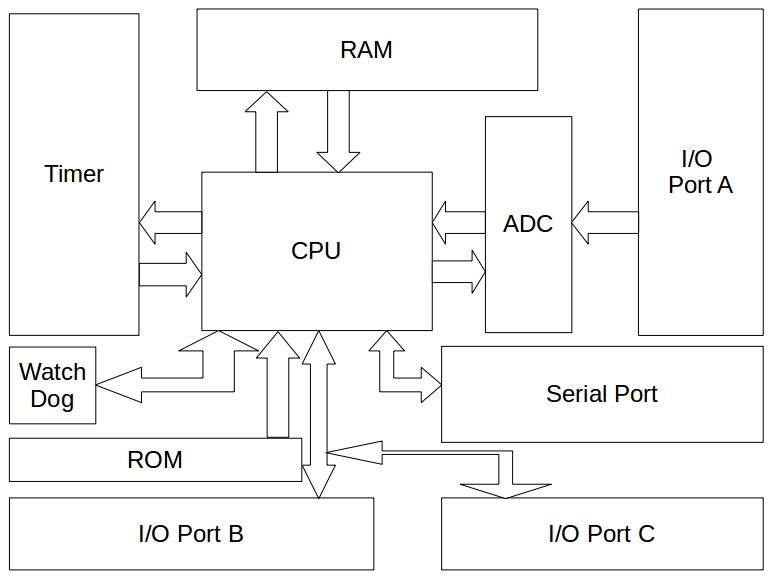
\includegraphics[scale=0.5]{microblock.jpg}  
\caption{Block Diagram of Microcontroller}
\end{figure}
\subsubsection*{Microcontroller block diagram explanation}
The explanation of the microcontroller\\cite{microcontroller} block diagram given above is as follows:
\begin{enumerate}
\item Central Processing Unit (CPU)\\
The CPU is the brain of any processing device of the microcontroller. It monitors and controls all operations that are performed on the Microcontroller units. The user has no control over the work of the CPU directly . It reads program written in ROM memory and executes them and do the expected task of that application. It performs all of the arithmetic and logic operations and controls the flow of execution of instructions.
\item Memory
Microcontroller requires a program which is a collection of instructions. This program tells microcontroller to do specific tasks. These programs require a memory on which these can be saved and read by Microcontroller to perform specific operations of a particular task. 
\begin{enumerate}
\item Random Access Memory(RAM)\\
The RAM holds the set of instructions (program). i.e. being executed by the CPU. It is a general purpose memory that can store data or programs. RAM is 'volatile', which means when the power is shut off, the contents of the memory is lost. Most personal computers have several megabytes of RAM. Most microcontrollers have some RAM built into them, but not very much. 256 bytes is a fairly common amount. Some have more, some have less. RAM is responsible for holding important data structures like 'stack'.\\
\item Read Only Memory(ROM)\\
ROM is Read Only Memory. This is typically memory that is programmed at the factory to have certain values. It cannot be changed, but it can be read as many times as wanted. ROM is typically used to store programs and data that doesn't change over time. In microcontrollers, it holds very important data and initialization about the microcontroller. It holds the monitor program and is written by the manufacturer. \\
\item Flash Memory
It is basically a Electrically Erasable Programmable Read Only Memory (EEPROM) and holds the program written by the user. The program can be erased or written here many times (specified by the manufacturer).\\
\end{enumerate}
\item Input/Output Ports\\
Normally microcontroller is used in embedded systems to control the operation of machines in the microcontroller. Therefore, to connect it to other machines, devices or peripherals we require I/O interfacing ports in the microcontroller interface. For example, microcontroller 8051 has 4 input, output ports to connect it to the other peripherals. Each port in a microcontroller is made up of n-pins (mostly 8 pins). Each pin can be configured as either input or output pin. If a pin is input pin, it accepts data from the device it is connected to. Similarly, if a pin is a output pin, it sends the data to the device it is connected to.
\item Analog to Digital Converter (ADC)\\
Most of the real world signals are analog in nature. But, a microcontroller is a digital device. Hence, it cannot process analog signals. This is why all microcontrollers have a built-in analog-to-digital converter. ADC digitizes an analog signal and gives it to the microcontroller for further processing. The conversion involves quantization of the input, so it necessarily introduces a small amount of error. Furthermore, instead of continuously performing the conversion, an ADC does the conversion periodically, sampling the input. The result is a sequence of digital values that have been converted from a continuous-time and continuous-amplitude analog signal to a discrete-time and discrete-amplitude digital signal.
\item Timers/Counters\\
Every microcontroller comes with one or more (sometimes many more) built-in timer/counters, and these are extremely useful. The term timer/counter itself reflects the fact that the underlying counter hardware can usually be configured to count either regular clock pulses (making it a timer) or irregular event pulses (making it a counter). The timer and counter functions in the microcontroller count in sync with the microcontroller clock. However, the counter only counts up to to either 256 (8 bit counter) or 65535 (16 bit counter). The microcontroller offers a quite useful feature called prescaling. Prescaling is a simplistic way for the counter to skip a certain number of clock ticks.\\
\item Interrupts\\
As its name suggests, Interrupt is a subroutine call that interrupts of the microcontrollers main operations or work and causes it to execute any other program, which is more important at the time of operation. The feature of Interrupt is very useful as it helps in case of emergency operations. An Interrupts gives us a mechanism to put on hold the ongoing operations, execute a subroutine and then again resumes to another type of operations.\\ 
\item Watchdog \\
A watchdog timer (WDT) is an embedded timing device that automatically prompts corrective action upon system malfunction detection. If software hangs or is lost, a WDT resets the system microcontroller via a 16-bit counter. A WDT is also known as a computer operating properly (COP) timer.\\
A WDT enables embedded system self-reliance in two ways:
\begin{enumerate}
\item Detects system glitches or errors, including programming errors, software hangs, code crashes or power surges. 
\item Resets operating systems and resumes normal program activity via the reset signal embedded in a CPU or specialized microcontroller chip. This reset process is also known as feeding the watchdog, kicking the dog, waking the watchdog or petting the dog. 
\end{enumerate}
\end{enumerate}
\subsubsection{Arduino UNO}
Arduino/Genuino Uno is a microcontroller board based on the ATmega328P. It has 14 digital input/output pins (of which 6 can be used as PWM outputs), 6 analog inputs, a 16 MHz quartz crystal, a USB connection, a power jack, an In-Circuit Serial Programming(ICSP) header and a reset button. It contains everything needed to support the microcontroller; simply connectable to a computer with a USB cable or can be powered with a AC-to-DC adapter or battery.Some of the important specification\cite{arduino} for Arduino UNO are: 
\begin{table}
\center
\begin{tabular}{ |p{5cm}|p{7cm}| }
\hline
\multicolumn{2}{|c|}{Specifications} \\
\hline
MicroController& ATMega328P \\
\hline
Operating Voltage& 5V\\
\hline
Input Voltage (recommended) & 7-12 V\\
\hline
Input Voltage (limit) &6-20V\\
\hline
Digital I/O pins &14(of which 6 provide PWM output) \\
\hline
PWM Digital I/O pins&6\\
\hline
Analag Input Pins & 6 \\
\hline
DC Current per I/O Pin	& 20 mA\\
\hline
DC Current for 3.3V Pin	& 50 mA\\
\hline
Flash Memory	& 32 KB (ATmega328P)
of which 0.5 KB used by bootloader\\
\hline
SRAM	& 2 KB (ATmega328P)\\
\hline
EEPROM	& 1 KB (ATmega328P)\\
\hline
Clock Speed	& 16 MHz\\
\hline
Length	& 68.6 mm\\
\hline
Width	& 53.4 mm\\
\hline
Weight	& 25 g\\
\hline
\end{tabular}
\caption{Arduino UNO Specifications}
\end{table}


